\chapter{动态模型}
\label{chap:pgm-dynamic}

一台设备连续两次报警，可能意味着故障正在持续，也可能来自传感器误报。前一次状态判断影响我们怎样理解下一次报警；后来的读数又可能改变我们对故障起点的判断。动态模型把设备状态的演化与传感器产生读数的机制分别表示，使历史判断可以与新证据逐步结合。本章研究这种递推怎样保存不确定性，以及它需要保留多少历史信息。

按时间组织有向分解后，递推预测只需把过去对未来有用的信息传到下一时刻。消元和消息传递正是完成这一压缩的工具（参考第~\ref{chap:pgm-directed}、\ref{chap:pgm-elimination}、\ref{chap:pgm-junction-tree}章）。本章先确定跨时刻传递的变量，再讨论有限概率表和高斯参数何时能精确保存这些信息。对于隐藏状态，推断还会提供后验统计量，让转移和观测参数可以从序列中学习。

这里的时间表示系统的采样时刻，或任务中有明确前后关系的序列位置。其他序列模型可能把不同对象放在时间轴上：序列条件随机场描述给定观测后的标签分布，适合条件预测（第~\ref{chap:pgm-energy-models}章）；扩散模型利用人为设定的噪声过程构造生成分布，其步数记录噪声过程的进展（第~\ref{chap:pgm-generative}章）。本章则围绕系统状态怎样演化、观测怎样反映状态展开。

\section{动态有向模型的共同形式}
\label{sec:pgm-dynamic-common}

设备在不同采样时刻往往遵循相同的依赖结构。把当前时刻内部的依赖和相邻时刻之间的依赖画成一个模板，再沿时间重复展开，就得到\term{动态有向图模型}（dynamic Bayesian network, DBN）。这一表示框架允许不同的状态空间与局部分布；隐马尔可夫模型和状态空间模型都可以借它组织。

把第$t$个时刻的变量放在同一个\term{时间切片}（time slice）内，记为随机向量$\bm{Y}_t=(Y_{t,1},\ldots,Y_{t,d})^\top$。其中$d$个变量可同时包含观测量和隐藏量。先考虑只连接相邻切片的模型，跨切片的边从$t-1$指向$t$。用$\operatorname{pa}^{-}(i)$记录节点$i$在上一切片的父节点索引，用$\operatorname{pa}^{0}(i)$记录当前切片的父节点索引。有向分解于是给出转移模板
\begin{equation}
  p(\bm{y}_t\mid\bm{y}_{t-1})
  =\prod_{i=1}^{d}
    p\bigl(y_{t,i}\mid
      \bm{y}_{t-1,\operatorname{pa}^{-}(i)},
      \bm{y}_{t,\operatorname{pa}^{0}(i)}\bigr).
  \label{eq:pgm-dynamic-two-slice}
\end{equation}
要求切片内部无环后，可以先按时间、再按切片内的拓扑序排列节点。这个顺序使任意有限长度$T$的展开都保持有向无环结构。序列的起点由初始分布$p(\bm{y}_1)$给定，后续切片再按转移模板生成。式~\eqref{eq:pgm-dynamic-two-slice}这段可重复的相邻切片结构称为\term{两切片动态有向图模型}（two-slice temporal Bayesian network, 2TBN）。

一种常用组织方式把影响未来的内部信息集中到潜状态$\bm{z}_t$，把传感器读数记为观测$\bm{x}_t$。状态可以是物理量，也可以是模型为预测而构造的变量。假设给定$\bm{z}_{t-1}$后，$\bm{z}_t$与更早状态条件独立；给定完整状态序列后，各时刻观测条件独立，且$\bm{x}_t$由$\bm{z}_t$产生。这两个局部机制组成\term{状态空间模型}（state space model, SSM）：
\begin{equation}
  \begin{aligned}
    p(\bm{z}_{1:T},\bm{x}_{1:T})
      &=p(\bm{z}_1)p(\bm{x}_1\mid\bm{z}_1)\\
      &\quad{}\times\prod_{t=2}^{T}
        p(\bm{z}_t\mid\bm{z}_{t-1})
        p(\bm{x}_t\mid\bm{z}_t).
  \end{aligned}
  \label{eq:pgm-dynamic-state-space}
\end{equation}
式~\eqref{eq:pgm-dynamic-state-space}把联合分布拆成初始、转移和观测三类因子，也为粒子滤波提供起点（第~\ref{sec:pgm-sampling-smc}节）。其中$\bm{z}_t$是潜状态，$\bm{x}_t$是观测；下文讨论这类分解何时能精确递推，并用于参数学习。记号$p$兼指概率质量函数和相对于相应测度的密度，离散状态的积分按求和理解。小写粗体表示向量；标量离散模型使用随机变量$Z_t,X_t$及取值$z_t,x_t$。图~\ref{fig:pgm-dynamic-template}展开了三个时刻，每个潜状态既产生当前观测，也传递未来所需的信息。允许观测间连边或更复杂切片内依赖的DBN则超出了这个状态空间特例。

\begin{figure}[htbp]
  \centering
  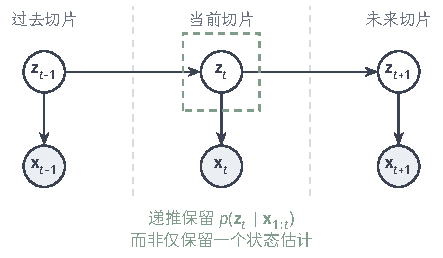
\includegraphics[width=74.997mm]{figures/06-probabilistic-graphical-models/04-models/tikz/pgm-dynamic-template/figure.pdf}
  \caption{状态空间模型在三个时刻的展开。空心节点为潜状态，填色节点为观测，竖直虚线分隔时间切片。当前潜状态的后验汇总过去证据，用于下一步预测；箭头表示生成依赖，平滑计算则沿状态链反向传递未来证据。}
  \label{fig:pgm-dynamic-template}
\end{figure}

递推需要保留多少历史，取决于状态怎样选择。\term{Markov假设}（Markov assumption）要求给定当前状态后，预测下一状态所需的信息已经齐备。对于$r$阶依赖$p(\bm{z}_t\mid\bm{z}_{t-r:t-1})$，可以把最近$r$个状态拼接成一个扩充状态，从而改写成一阶模型，代价是扩大状态空间。观测只间接反映内部状态，因此观测历史仍可能持续改变当前状态的后验，即使潜状态满足一阶Markov性。

设备每次按相同规则升温，温度分布仍会从冷启动逐渐向高温移动。这里保持的是局部机制：\term{时间齐次性}（time homogeneity）要求转移核不随$t$改变；\term{参数共享}（parameter sharing）表示不同位置复用同一组转移或观测参数。共享参数的条件分布若还依赖时间或已知外部输入，取值仍可随时刻变化。\term{严格平稳性}（strict stationarity）约束的则是整个过程，要求任意有限组时刻的联合分布在整体平移后保持不变。齐次Markov链从平稳分布初始化时，才得到这样的平稳过程。

将过去变量消去后，需要把哪些信息留给未来？所有跨越时间分界的依赖经过的变量集合称为\term{时间接口}（temporal interface）。一阶状态空间模型只需保留$\bm{z}_t$的后验，因为给定这个状态，过去与未来被分开。一般DBN可以保留当前切片中有下一切片子节点的变量及其联合分布。过去证据可能让这些变量相关，联合分布因此包含单独边缘没有保存的信息。计算代价取决于离散接口的联合配置数，或连续后验的表示复杂度，这也是消元中诱导宽度的重要来源（第~\ref{chap:pgm-elimination}章）。Koller和Friedman详细讨论了图模板、时间接口与精确推断的关系\scite{pgm-koller2009}

设备监测提出三类查询。\term{预测}（prediction）给出$p(\bm{z}_{t+h}\mid\bm{x}_{1:t})$或$p(\bm{x}_{t+h}\mid\bm{x}_{1:t})$，其中$h\geq1$，用于判断未来状态或读数。\term{滤波}（filtering）给出$p(\bm{z}_t\mid\bm{x}_{1:t})$，用于收到新读数后判断当前状态。\term{平滑}（smoothing）给出$p(\bm{z}_t\mid\bm{x}_{1:T})$，其中$t<T$，用于事后结合未来证据重建过去。固定间隔平滑读取长度为$T$的整段数据；固定滞后平滑只等待预定步数的未来观测，适合允许延迟的状态判断。

重建整段工况还可能需要\term{最可能状态序列}（most probable state sequence），即让$p(\bm{z}_{1:T}\mid\bm{x}_{1:T})$达到最大的整条路径。对全部潜状态求最大值得到MPE查询；保留部分状态求最大值、其余状态求和或积分，则得到边缘MAP（第~\ref{chap:pgm-elimination}章）。逐时刻取平滑边缘的最大项，对应按各位置误判数评价的决策；整条路径优化评价的是联合概率，两种目标可能选择不同结果。连续状态的路径最优以所选坐标和基准测度下的后验密度为准。

预测和滤波可以从当前后验逐步计算，平滑则在此基础上加入未来证据。记上一步滤波分布为$f_{t-1}(\bm{z}_{t-1})=p(\bm{z}_{t-1}\mid\bm{x}_{1:t-1})$。将它与转移分布结合并消去旧状态，得到当前预测；再乘当前观测似然并归一化，得到
\begin{equation}
  \begin{aligned}
    f_t^{-}(\bm{z}_t)
      &=\int p(\bm{z}_t\mid\bm{z}_{t-1})
        f_{t-1}(\bm{z}_{t-1})\,\mathrm{d}\bm{z}_{t-1},\\
    c_t
      &=\int p(\bm{x}_t\mid\bm{z}_t)
        f_t^{-}(\bm{z}_t)\,\mathrm{d}\bm{z}_t,\\
    f_t(\bm{z}_t)
      &=\frac{p(\bm{x}_t\mid\bm{z}_t)
        f_t^{-}(\bm{z}_t)}{c_t}.
  \end{aligned}
  \label{eq:pgm-dynamic-bayes-filter}
\end{equation}
第一次预测取$f_1^{-}=p(\bm{z}_1)$；每个归一化量$c_t$需有限且为正。它同时等于$c_t=p(\bm{x}_t\mid\bm{x}_{1:t-1})$，所以$\log p(\bm{x}_{1:T})=\sum_{t=1}^{T}\log c_t$给出整段观测的对数似然。一次递推因而既更新状态判断，也累计训练和模型比较需要的分数。有限状态与线性高斯模型的优势在于，这些积分或求和可以精确计算，结果仍有固定大小的表示。

\section{离散状态演化模型}
\label{sec:pgm-dynamic-discrete}

如果每次巡检都能可靠记录设备的正常或异常状态，训练序列就直接给出了状态转移。用$Z_t\in\{1,\ldots,K\}$表示有限状态，$\pi_i=p(Z_1=i)$表示初始概率。齐次转移矩阵$\bm{A}\in\mathbb{R}^{K\times K}$的元素为
\[
  a_{i,j}=p(Z_t=j\mid Z_{t-1}=i),\qquad
  a_{i,j}\geq0,\quad \sum_{j=1}^{K}a_{i,j}=1.
\]
矩阵每一行列出从一个当前状态到各下一状态的概率，非负且总和为一。本节考虑有限状态、离散时间和齐次转移，初始概率$\bm\pi$按列向量记录（Markov关系参考\BookSectionRef{sec:rv-markov}{第一卷“数学准备”的Markov关系小节}）。

把当前状态分布记为概率列向量$\bm{q}_t$。对随机状态$Z_t$求和，下一步分布满足$\bm{q}_{t+1}=\bm{A}^{\top}\bm{q}_t$。重复这一计算便得到
\begin{equation}
  \bm{q}_{t+h}=(\bm{A}^{\top})^h\bm{q}_t,\qquad
  p(Z_{t+h}=j\mid Z_t=i)=(\bm{A}^h)_{i,j}.
  \label{eq:pgm-dynamic-markov-prediction}
\end{equation}
两步转移中的$\sum_k a_{i,k}a_{k,j}$累加了经过各个中间状态的路径概率。继续累加中间状态，就得到$h$步矩阵幂；转置来自概率列向量与按行定义的转移矩阵之间的约定。

\begin{example}[两状态设备的多步预测]
  \label{ex:pgm-dynamic-markov}
  为单独展示多步预测，设状态$1$为正常、状态$2$为异常，采用下面的人工参数。它与四节点报警模型及例~\ref{ex:pgm-sampling-filter}分别设定，后面的发射概率也将另给：
  \[
    \bm{\pi}=\begin{pmatrix}0.8\\0.2\end{pmatrix},\qquad
    \bm{A}=
    \begin{pmatrix}0.9&0.1\\0.2&0.8\end{pmatrix}.
  \]
  从确定正常的状态出发，下一步异常概率为$0.1$；两步后需要累加先正常后异常和先异常后异常两条路径，得到$0.9\times0.1+0.1\times0.8=0.17$。当前异常概率为$u_t$时，递推为
  \[
    u_{t+1}=0.1(1-u_t)+0.8u_t=0.1+0.7u_t.
  \]
  解得$u_{t+h}=1/3+0.7^h(u_t-1/3)$。初始偏差随预测步数按几何因子衰减，异常概率趋向$1/3$；这个极限由正常进入异常和异常退出两种转移共同决定。
\end{example}

例~\ref{ex:pgm-dynamic-markov}的极限是平稳分布$(2/3,1/3)^\top$，满足$\bm A^\top\bm\pi_\star=\bm\pi_\star$。平稳分布给出转移后保持不变的分布；从任意初态是否趋向它，还取决于链的长期行为条件。时间平均又涉及沿同一条路径累积的观测量（参考\BookSectionRef{sec:stoch-markov-long-run-average}{第一卷“数学准备”的Markov链长期行为小节}）。下面转向如何从数据估计转移概率，以及状态隐藏时怎样推断。

可见状态的参数学习可以直接使用转移计数。令$n_{i,j}$为训练序列中$i\to j$的次数，转移对数似然为$\sum_{i,j}n_{i,j}\log a_{i,j}$。在各行总和为$1$的约束下最大化，得到$\widehat a_{i,j}=n_{i,j}/\sum_k n_{i,k}$。从未访问的行会出现$0/0$，意味着数据没有给出该行的信息，可用先验或保留旧值处理。多条独立序列分别计数后汇总，序列之间的接缝不计作转移；初始分布则只统计各序列首状态。

设备内部的健康状态通常隐藏在报警、温度等读数之后。用一个有限状态链描述内部演化，再给每个状态指定产生读数的分布，就得到\term{隐马尔可夫模型}（hidden Markov model, HMM）。其中的\term{发射分布}（emission distribution）描述给定状态后的观测，记$b_j(x)=p(x\mid Z_t=j)$为它在$x$处的概率质量或密度。联合分布为
\begin{equation}
  p(z_{1:T},x_{1:T})
    =\pi_{z_1}b_{z_1}(x_1)
      \prod_{t=2}^{T}a_{z_{t-1},z_t}b_{z_t}(x_t).
  \label{eq:pgm-dynamic-hmm}
\end{equation}
HMM的隐藏状态取离散值，观测则可以是Bernoulli报警，也可以是服从状态相关高斯密度的温度。与独立混合模型相比，它用转移分布连接相邻潜类别，使前一时刻的工况影响下一时刻的成分选择（第~\ref{chap:pgm-static-directed}章）。

计算观测似然$p(x_{1:T})$时，直接枚举隐藏路径要遍历$K^T$个配置。具有同一末状态的前缀可以共享未来计算，因此先把它们的联合概率加在一起。这个和就是未归一化前向消息$\alpha_t(j)=p(x_{1:t},Z_t=j)$。它满足
\[
  \alpha_t(j)
    =b_j(x_t)\sum_i
      p(x_{1:t-1},Z_{t-1}=i)a_{i,j}
\]
据此前向消息可递推为
\begin{equation}
  \begin{aligned}
    \alpha_1(j)&=\pi_jb_j(x_1),\\
    \alpha_t(j)&=b_j(x_t)\sum_{i=1}^{K}
      \alpha_{t-1}(i)a_{i,j},\\
    p(x_{1:T})&=\sum_j\alpha_T(j).
  \end{aligned}
  \label{eq:pgm-dynamic-forward}
\end{equation}
递推每次消去$Z_{t-1}$，更早路径的贡献已汇总到$\alpha_{t-1}$中。从初始联合概率出发，这一步始终保持$\alpha_t$的概率含义，也说明了前缀合并为何精确。将各状态的消息归一化，$\alpha_t(j)/\sum_i\alpha_t(i)$就是滤波概率。

事后重建早期状态，需要把未来证据压缩成一条反向消息。定义$\beta_t(i)=p(x_{t+1:T}\mid Z_t=i)$；末时刻没有未来观测，故$\beta_T(i)=1$。对下一状态边缘化可得
\begin{equation}
  \begin{aligned}
    \beta_t(i)&=\sum_{j=1}^{K}
      a_{i,j}b_j(x_{t+1})\beta_{t+1}(j),\\
    \gamma_t(i)&:=p(Z_t=i\mid x_{1:T})
      =\frac{\alpha_t(i)\beta_t(i)}{L},\\
    \xi_t(i,j)&:=p(Z_t=i,Z_{t+1}=j\mid x_{1:T})\\
      &=\frac{\alpha_t(i)a_{i,j}b_j(x_{t+1})
        \beta_{t+1}(j)}{L},
  \end{aligned}
  \label{eq:pgm-dynamic-backward}
\end{equation}
这里$L=p(x_{1:T})>0$为整段观测似然。给定$Z_t$后，过去与未来观测条件独立，因而$\alpha_t\beta_t$可以合并两部分证据，再由同一个似然归一化。\term{前向--后向算法}（forward--backward algorithm）据此分别压缩过去和未来：$\gamma_t$给出单时刻平滑，$\xi_t$保存相邻状态的联合后验，供转移参数学习使用。

为减少长序列连乘造成的数值下溢，每一步都把前向消息归一化，记$\widehat\alpha_t(j)=p(Z_t=j\mid x_{1:t})$，并保存未归一化消息的总和$c_t$。后向缩放与它配合：令$\widehat\beta_T=1$，将$\sum_j a_{i,j}b_j(x_{t+1})\widehat\beta_{t+1}(j)$除以$c_{t+1}$。这样$\gamma_t(i)=\widehat\alpha_t(i)\widehat\beta_t(i)$，$\xi_t$也使用$c_{t+1}$归一化。另一种实现是在对数域稳定求和。若$c_t=0$，当前观测前缀落在模型支撑之外，应终止更新并检查分布设定或数值计算。

\begin{algorithm}[缩放的HMM前向--后向递推]
  \label{alg:pgm-dynamic-forward-backward}
  \begin{algorithmic}[1]
    \Require $\bm{\pi},\bm{A},b_j$与观测$x_{1:T}$，$T\geq1$
    \Ensure 似然对数、平滑概率$\gamma_t$与成对概率$\xi_t$
    \State $u_1(j)\gets\pi_jb_j(x_1)$，$c_1\gets\sum_j u_1(j)$
    \State 若$c_1=0$，报告观测不在模型支撑内并终止
    \State $\widehat\alpha_1(j)\gets u_1(j)/c_1$
    \For{$t=2,\ldots,T$}
      \State $u_t(j)\gets b_j(x_t)\sum_i\widehat\alpha_{t-1}(i)a_{i,j}$
      \State $c_t\gets\sum_j u_t(j)$；若$c_t=0$则报告并终止
      \State $\widehat\alpha_t(j)\gets u_t(j)/c_t$
    \EndFor
    \State $\widehat\beta_T(i)\gets1$，$\gamma_T(i)\gets\widehat\alpha_T(i)$
    \For{$t=T-1,\ldots,1$}
      \State $\widehat\beta_t(i)\gets
        \sum_j a_{i,j}b_j(x_{t+1})\widehat\beta_{t+1}(j)/c_{t+1}$
      \State $\gamma_t(i)\gets\widehat\alpha_t(i)\widehat\beta_t(i)$
      \State $\xi_t(i,j)\gets
        \widehat\alpha_t(i)a_{i,j}b_j(x_{t+1})
        \widehat\beta_{t+1}(j)/c_{t+1}$
    \EndFor
    \State 返回$\sum_t\log c_t$及上述后验统计量
  \end{algorithmic}
\end{algorithm}

密集转移下，算法~\ref{alg:pgm-dynamic-forward-backward}每步遍历状态对，时间成本为$O(TK^2)$，再加发射概率求值。在线滤波只保留一条消息，工作内存为$O(K)$；平滑保存全部前向消息，需要$O(TK)$内存。为EM计算转移计数时，可以逐步累加$\xi_t$，省去$T$张$K\times K$表的存储。若转移图稀疏，计算只遍历允许的边，成本随这些边的数量变化。

\begin{example}[报警证据怎样改变过去的判断]
  \label{ex:pgm-dynamic-hmm}
  沿用例~\ref{ex:pgm-dynamic-markov}的$\bm{\pi}$和$\bm{A}$。记$X_t=1$为报警，另设教学发射概率$b_1(1)=0.1$、$b_2(1)=0.7$，表示异常工况更易报警。观测$x_{1:3}=(0,1,1)$产生如下前向消息：
  \[
    \begin{aligned}
      \bm{\alpha}_1&=(0.72,0.06)^\top,\\
      \bm{\alpha}_2&=(0.066,0.084)^\top,\\
      \bm{\alpha}_3&=(0.00762,0.05166)^\top.
    \end{aligned}
  \]
  第二步的正常权重为$(0.72\times0.9+0.06\times0.2)\times0.1=0.066$：先汇总两种前状态转到正常的贡献，再乘正常时报警的概率。总似然为$0.05928$，后向消息依次为$\bm{\beta}_3=(1,1)^\top$、$\bm{\beta}_2=(0.16,0.58)^\top$和$\bm{\beta}_1=(0.055,0.328)^\top$。第一个时刻的异常滤波概率是$0.06/0.78\approx0.0769$，加入后续证据后的异常平滑概率为$0.06\times0.328/0.05928\approx0.3320$。连续报警增加了此前已经异常、第一次却未报警这一解释的权重。
\end{example}

表~\ref{tab:pgm-dynamic-hmm-example}把同一序列的两类判断并列。这里，两次报警及异常状态的持续性共同提高了早期异常的后验概率；在其他观测序列下，未来证据也可以降低这个概率。

\begin{table}[htbp]
  \centering
  \begin{tabular}{ccrr}
    \toprule
    时刻$t$ & 报警$x_t$ & 异常滤波概率 & 异常平滑概率 \\
    \midrule
    $1$ & $0$ & $0.076923$ & $0.331984$ \\
    $2$ & $1$ & $0.560000$ & $0.821862$ \\
    $3$ & $1$ & $0.871457$ & $0.871457$ \\
    \bottomrule
  \end{tabular}
  \caption{同一人工设备序列的异常后验。滤波列逐步读取当前及过去观测，平滑列使用完整$x_{1:3}$；最后一个时刻的证据范围相同，因而两列重合。}
  \label{tab:pgm-dynamic-hmm-example}
\end{table}

寻找联合概率最大的路径时，每个末状态只需保留最优前缀及其前驱。记$\delta_t(j)$为以$j$结尾的路径中最大的联合概率$p(z_{1:t},x_{1:t})$，用前驱表保存最大值来自哪一个状态。\term{Viterbi算法}（Viterbi algorithm）据此递推：
\begin{equation}
  \begin{aligned}
    \delta_1(j)&=\pi_jb_j(x_1),\\
    \delta_t(j)&=b_j(x_t)\max_i
      \{\delta_{t-1}(i)a_{i,j}\},\\
    \psi_t(j)&\in\argmax_i
      \{\delta_{t-1}(i)a_{i,j}\}.
  \end{aligned}
  \label{eq:pgm-dynamic-viterbi}
\end{equation}
先选末状态$z_T^\star\in\argmax_j\delta_T(j)$，再按$z_t^\star=\psi_{t+1}(z_{t+1}^\star)$回溯；平局可按最小索引处理。当末状态固定时，未来因子对全部前缀相同，所以保留较优前缀足以保留整体最优解。密集转移的时间成本仍为$O(TK^2)$，回溯表占$O(TK)$。对数得分实现可避免路径概率连乘下溢，并以$-\infty$表示禁止的转移。

例~\ref{ex:pgm-dynamic-hmm}的最优路径是$(1,2,2)$，联合概率为$0.8\times0.9\times0.1\times0.7\times0.8\times0.7=0.028224$，给定观测后的路径概率约为$0.4761$，其余概率仍分散在其他路径上。逐位置选择与联合选择的差别可看另一个两时刻分布：令$(1,1),(1,2),(2,1),(2,2)$的概率为$0.40,0.25,0.01,0.34$，两个边缘分别选择$1$和$2$，组成的$(1,2)$却不如联合最优$(1,1)$。取初始分布$(0.65,0.35)$并按上述联合概率确定条件转移，即可构造这个Markov例子。

隐藏状态没有实际可读的转移计数，却可以按各路径的后验概率累计期望计数。\term{Baum--Welch算法}（Baum--Welch algorithm）用这一思路在HMM上执行EM：E步计算当前参数下的$\gamma_t,\xi_t$，M步根据这些软计数拟合初始、转移和发射分布。当前参数记为$\bm{\theta}^{(k)}$，期望完全数据对数似然为
\begin{equation}
  \begin{aligned}
    \mathcal{Q}(\bm{\theta}\mid\bm{\theta}^{(k)})
      &=\sum_i\gamma_1(i)\log\pi_i\\
      &\quad{}+\sum_{t=1}^{T-1}\sum_{i,j}
        \xi_t(i,j)\log a_{i,j}\\
      &\quad{}+\sum_{t=1}^{T}\sum_j
        \gamma_t(j)\log b_j(x_t).
  \end{aligned}
  \label{eq:pgm-dynamic-hmm-em-objective}
\end{equation}
在一次M步中固定旧参数算出的后验权重，只调整对数内的候选参数。对$a_{i,j}$施加逐行归一化约束，一阶条件给出$a_{i,j}\propto\sum_t\xi_t(i,j)$。由于$\sum_j\xi_t(i,j)=\gamma_t(i)$，更新可写为
\begin{equation}
  \begin{aligned}
    \pi_i^{(k+1)}&=\gamma_1(i),\\
    a_{i,j}^{(k+1)}
      &=\frac{\sum_{t=1}^{T-1}\xi_t(i,j)}
        {\sum_{t=1}^{T-1}\gamma_t(i)},\\
    b_j^{(k+1)}(v)
      &=\frac{\sum_{t=1}^{T}
        \gamma_t(j)\mathbf{1}\{x_t=v\}}
        {\sum_{t=1}^{T}\gamma_t(j)}.
  \end{aligned}
  \label{eq:pgm-dynamic-baum-welch}
\end{equation}
类别发射用最后一行的期望频数更新。高斯发射则按$\sum_t\gamma_t(j)\bm{x}_t/\sum_t\gamma_t(j)$更新均值，再围绕这个新均值累计加权残差外积，得到协方差。多条独立序列先分别计算统计量，再相加更新转移和发射；初始概率使用各序列$\gamma_1$的平均。

本例得到$\xi_1(1,2)=0.72\times0.1\times0.7\times0.58/0.05928\approx0.493117$和$\xi_2(1,2)\approx0.077935$。一次M步将$a_{1,2}$更新为$(0.493117+0.077935)/(0.668016+0.178138)\approx0.674880$，两个状态的报警概率变为$0.314642$和$0.836082$。只有三次读数时，估计容易随证据显著变化。训练中可比较多组初值，用似然相对增量与迭代上限控制停止，再用独立序列或时间隔离的验证段评价这些参数的预测表现。

精确E步与提高$\mathcal Q$的M步使观测似然单调不降（第~\ref{chap:pgm-parameter-learning}章），它评价的是同一训练数据上的目标进展。全局最优需要进一步的优化条件，状态解释依赖可识别性，测试预测则需要独立数据检验。某个更新分母为零时，该轮后验没有访问相应状态，软计数对参数不提供信息。正初始化、结构约束和先验可以处理部分退化，估计的可识别范围仍由数据与模型共同决定。

给隐藏状态重新编号，同时置换$\bm{\pi}$、$\bm{A}$的行列和对应发射分布，会得到完全相同的观测似然。这种\term{标签交换}（label switching）使状态编号只能在选定约定下解释。发射分布接近时，数据也难以区分状态；全部发射相同且按式~\eqref{eq:pgm-dynamic-hmm}生成时，状态路径求和后，观测分布中的转移信息完全消失。选择状态数$K$时，增加$K$可能复制已有状态，也可能补偿持续时间假设的偏差。应结合验证预测似然、持续时间解释和后验占用检查模型；使用常规信息准则还需考虑潜变量模型的奇异性与可识别性条件。Murphy的教材系统介绍了HMM推断、学习和模型选择\scite{pgm-murphy2012}

实际系统可能需要更长历史来预测转移。若下一状态依赖最近$r$个状态，模型成为\term{高阶HMM}（higher-order HMM）。把$(Z_{t-r+1},\ldots,Z_t)$拼成扩充状态后，仍可执行动态规划。一次转移移去最早状态、加入新状态，所以每个扩充状态只有$K$个合法后继，计算成本为$O(TK^{r+1})$。虽然共有$K^r$个扩充状态，转移图保留了稀疏移位结构；消息本身仍需记录$K^r$个配置。

设备在一种工况中已经运行的时长，也可能影响退出概率。普通HMM进入状态$i$后，每步以固定概率$a_{i,i}<1$继续停留，因此连续停留时长$D$服从
\begin{equation}
  p(D=\ell\mid i)=(a_{i,i})^{\ell-1}(1-a_{i,i}),
  \qquad
  \mathbb{E}[D\mid i]=\frac{1}{1-a_{i,i}}.
  \label{eq:pgm-dynamic-geometric-duration}
\end{equation}
其中$\ell-1$次自转移后接一次退出，产生\term{几何持续时间}（geometric duration）。退出概率与已经停留的时长无关，本例正常工况的平均持续时间为$10$步。如果设备必须运行至少$5$步才允许退出，就需要让持续时间本身进入模型。

为工况另给持续时间分布$g_j(\ell)$，得到\term{显式持续时间模型}（explicit-duration model）。\term{隐半Markov模型}（hidden semi-Markov model, HSMM）据此以片段为单位：片段内部状态固定，边界处按$\widetilde a_{i,j}$转移。常用$\widetilde a_{j,j}=0$使相邻片段对应不同状态。状态$j$的片段长$\ell$、结束于$t$时，条件观测似然为$B_j(t,\ell)=\prod_{s=t-\ell+1}^{t}b_j(x_s)$。这里假设序列从新片段开始，$g_j$在$\{1,\ldots,D_{\max}\}$上归一化。记$F_t(j)$为观测前缀与一个$j$片段恰在$t$结束的联合概率，$G_s(j)$为前$s$步观测与下一片段进入$j$的联合权重，递推为
\begin{equation}
  \begin{aligned}
    G_0(j)&=\pi_j,\\
    G_s(j)&=\sum_{i\ne j}
      F_s(i)\widetilde a_{i,j},\qquad s\geq1,\\
    F_t(j)&=\sum_{\ell=1}^{\min(t,D_{\max})}
      g_j(\ell)B_j(t,\ell)G_{t-\ell}(j).
  \end{aligned}
  \label{eq:pgm-dynamic-hsmm}
\end{equation}
每一项把前一片段的权重、当前片段的长度概率和观测似然相乘，再对可能长度求和。采样固定在$T$停止时，最后一段可能仍在持续，形成右删失。用存活概率$\overline g_j(\ell)=p(D\geq\ell\mid j)$保留这一信息，整体似然为
\[
  p(x_{1:T})=\sum_j\sum_{\ell=1}^{\min(T,D_{\max})}
    \overline g_j(\ell)B_j(T,\ell)G_{T-\ell}(j)
\]
这一式子包含在$T$结束和越过终点继续持续的片段。若采样也从片段中途开始，需另外指定初始剩余时长分布。预计算片段发射概率并缓存$G_s(j)$后，常规成本从$O(TD_{\max}K^2)$降到$O(TK^2+TD_{\max}K)$，其中先汇总边界转移，再枚举片段长度；这一分离依赖发射条件独立及持续时间不依赖前驱状态。将无限支撑持续时间截断会引入额外误差。EM相应累计片段、边界转移和持续时间的后验期望计数。

设备健康状态和传感器工作状态也可能分别演化，却共同决定报警。\term{因子HMM}（factorial HMM）用多条隐藏链表示这些过程。记$Z_{t,m}$为第$m$条链的状态，$m=1,\ldots,M$，模型规定
\begin{equation}
  \begin{aligned}
    p(\bm{z}_t\mid\bm{z}_{t-1})
      &=\prod_{m=1}^{M}
        p(z_{t,m}\mid z_{t-1,m}),\\
    p(\bm{x}_t\mid\bm{z}_t)
      &=p(\bm{x}_t\mid z_{t,1},\ldots,z_{t,M}).
  \end{aligned}
  \label{eq:pgm-dynamic-factorial}
\end{equation}
先验转移分别作用于各条链，共同观测则把它们连接起来。例如，同一次报警可以由设备异常或传感器异常解释，观测后两种解释的概率彼此关联。每链$K$个状态时，精确联合消息包含$K^M$种配置；按各维依次收缩转移乘积，可用约$O(MK^{M+1})$成本完成一步预测，仍随链数指数增长。结构化变分保留链内时间依赖并近似链间相关，采样也可以估计E步统计量。Ghahramani和Jordan系统分析了因子HMM的这种后验耦合\scite{pgm-dynamic-ghahramani1997}

\section{连续与混合状态演化模型}
\label{sec:pgm-dynamic-continuous}

温度偏移和位置需要连续数值表示；若用有限状态格子追踪，分辨率越高，HMM的状态数越大。保留连续状态后，还可以借助高斯族完成精确递推：线性变换和高斯条件化都保持高斯形式。\term{线性高斯状态空间模型}（linear Gaussian state space model, LGSSM）采用高斯初态、线性映射和独立高斯扰动，使整个有限序列成为联合高斯。

设潜状态$\bm{z}_t\in\mathbb{R}^{q}$、观测$\bm{x}_t\in\mathbb{R}^{p}$。对于齐次参数且无外部输入的系统，基本方程为
\begin{equation}
  \begin{aligned}
    \bm{z}_1&\sim\mathcal{N}(\bm{m}_0,\bm{P}_0),\\
    \bm{z}_t&=\bm{A}\bm{z}_{t-1}+\bm{\varepsilon}_t,
      &\bm{\varepsilon}_t&\sim\mathcal{N}(\bm{0},\bm{Q}),\\
    \bm{x}_t&=\bm{C}\bm{z}_t+\bm{\eta}_t,
      &\bm{\eta}_t&\sim\mathcal{N}(\bm{0},\bm{R}).
  \end{aligned}
  \label{eq:pgm-dynamic-lgssm}
\end{equation}
矩阵$\bm{A}\in\mathbb{R}^{q\times q}$作用于状态，$\bm{C}\in\mathbb{R}^{p\times q}$把状态映射为观测均值；$\bm{Q}$、$\bm{R}$分别描述过程和测量噪声。噪声相互独立、跨时刻独立，并与初始状态独立。这里$\bm{A}$是线性映射，其行和可以偏离$1$，与离散转移表的含义不同。先取$\bm{P}_0,\bm{Q},\bm{R}$正定，以便使用密度和逆矩阵；退化情形需在支撑子空间内处理。已知控制量$\bm{u}_t$可以通过$\bm{B}\bm{u}_t$进入状态方程，时变矩阵也可按时刻递推，保留的是线性高斯结构。

用$\bm{m}_{t\mid s}=\mathbb{E}[\bm{z}_t\mid\bm{x}_{1:s}]$和$\bm{P}_{t\mid s}=\operatorname{Cov}(\bm{z}_t\mid\bm{x}_{1:s})$记录后验均值和协方差。在上述线性高斯条件下，这两项完整确定状态后验（参考\BookSectionRef{sec:dynamical-kalman-rts}{第一卷“数学准备”的线性高斯滤波与平滑小节}）。对本章的状态和观测$\bm z_t,\bm x_t$，先将旧滤波分布经线性转移传播，得到
\begin{equation}
  \begin{aligned}
    \bm{m}_{t\mid t-1}&=\bm{A}\bm{m}_{t-1\mid t-1},\\
    \bm{P}_{t\mid t-1}
      &=\bm{A}\bm{P}_{t-1\mid t-1}\bm{A}^{\top}
        +\bm{Q}.
  \end{aligned}
  \label{eq:pgm-dynamic-kalman-predict}
\end{equation}
起点$t=1$使用给定初始分布，即$\bm{m}_{1\mid0}=\bm{m}_0$、$\bm{P}_{1\mid0}=\bm{P}_0$。此后的预测协方差把两种来源相加：旧状态的不确定性经过线性映射传播，过程噪声贡献本步新增的不确定性。

预测观测的协方差为$\bm S_t=\bm C\bm P_{t\mid t-1}\bm C^\top+\bm R$。实际读数与预测均值之差称为新息，对状态与观测的联合高斯分布作条件化，得到
\begin{equation}
  \begin{aligned}
    \bm{e}_t&=\bm{x}_t-\bm{C}\bm{m}_{t\mid t-1},\\
    \bm{K}_t&=\bm{P}_{t\mid t-1}\bm{C}^{\top}\bm{S}_t^{-1},\\
    \bm{m}_{t\mid t}
      &=\bm{m}_{t\mid t-1}+\bm{K}_t\bm{e}_t,\\
    \bm{P}_{t\mid t}
      &=\bm{P}_{t\mid t-1}
        -\bm{K}_t\bm{S}_t\bm{K}_t^{\top}.
  \end{aligned}
  \label{eq:pgm-dynamic-kalman-update}
\end{equation}
新息$\bm e_t$给出测量与预测的偏差，Kalman增益$\bm K_t$把这个偏差转成状态均值的修正。在线性高斯及独立噪声条件下，更新给出精确后验；仅有二阶矩时，它可用于最佳线性估计，一般非高斯后验的完整形状还需要其他信息。实现增益时可解线性方程，协方差则可用Joseph形式或平方根递推保持数值稳定（参考\BookEquationRef{eq:dynamical-kalman-joseph-form}{第一卷“数学准备”的Joseph协方差形式}）。缺失机制可忽略时，无观测的一步只做预测，部分缺失则取$\bm C$的实际观测行与$\bm R$的相应子矩阵；可忽略条件见第~\ref{chap:pgm-parameter-learning}章。

同一个预测计算给出观测密度$\mathcal N(\bm{x}_t;\bm{C}\bm{m}_{t\mid t-1},\bm{S}_t)$。把各步预测密度的对数累加，得到
\begin{equation}
  \log p(\bm{x}_{1:T})
    =-\frac12\sum_{t=1}^{T}
      \left[
        p\log(2\pi)+\log|\bm{S}_t|
        +\bm{e}_t^\top\bm{S}_t^{-1}\bm{e}_t
      \right].
  \label{eq:pgm-dynamic-kalman-likelihood}
\end{equation}
对数似然同时衡量预测偏差和预测不确定性，可用于拟合参数与评价观测预测。完整观测、密集矩阵下，每步常规成本为$O(q^3+p^3+q^2p+qp^2)$；在线状态存储为$O(q^2)$，观测计算另外需要约$p^2+pq$大小的矩阵。状态与观测维度固定时，总成本随序列长度$T$线性增加。

学习参数需要整段观测下的状态矩，因此在前向滤波之后反向传播未来证据。RTS平滑用下面的增益，将下一状态的平滑修正传回当前状态：
\[
  \bm{J}_t=\bm{P}_{t\mid t}\bm{A}^{\top}
    \bm{P}_{t+1\mid t}^{-1}.
\]
在线性高斯条件下，反向条件均值及协方差给出精确递推（参考\BookTheoremRef{thm:dynamical-rts-smoother}{第一卷“数学准备”的RTS平滑定理}）：
\begin{equation}
  \begin{aligned}
    \bm{m}_{t\mid T}
      &=\bm{m}_{t\mid t}
        +\bm{J}_t(\bm{m}_{t+1\mid T}
          -\bm{m}_{t+1\mid t}),\\
    \bm{P}_{t\mid T}
      &=\bm{P}_{t\mid t}
        +\bm{J}_t(\bm{P}_{t+1\mid T}
          -\bm{P}_{t+1\mid t})\bm{J}_t^\top.
  \end{aligned}
  \label{eq:pgm-dynamic-rts}
\end{equation}
从$t=T$的滤波结果初始化，依次处理$t=T-1,\ldots,1$。逆向增益使用前向滤波协方差，因而未来证据沿各时刻已建立的条件关系传回。保存前向均值、协方差和预测量后，常规实现需$O(Tq^2)$存储，反向过程增加$O(Tq^3)$的密集矩阵计算。

学习转移映射还需要相邻状态的联合矩。反向条件均值的残差与$\bm{z}_{t+1}$条件不相关，所以其滞后一阶协方差为
\begin{equation}
  \begin{aligned}
    \bm{P}_{t,t-1\mid T}
      &:=\operatorname{Cov}(\bm{z}_t,\bm{z}_{t-1}
        \mid\bm{x}_{1:T})\\
      &=\bm{P}_{t\mid T}\bm{J}_{t-1}^{\top},
      \qquad t=2,\ldots,T.
  \end{aligned}
  \label{eq:pgm-dynamic-lag-covariance}
\end{equation}
转置决定这里的方向：$\bm{J}_{t-1}\bm{P}_{t\mid T}$给出$\operatorname{Cov}(\bm{z}_{t-1},\bm{z}_{t}\mid\bm{x}_{1:T})$，与展示式互为转置。相邻状态仍共享后验不确定性，学习动态关系时，需要把这项协方差与均值外积一起计入。

\begin{example}[温度偏移的滤波、平滑与二阶矩]
  \label{ex:pgm-dynamic-kalman}
  另设一个以摄氏度为单位的人工温度偏移模型：$Z_1\sim\mathcal{N}(0,1)$、$Z_2=Z_1+\varepsilon_2$、$X_t=Z_t+\eta_t$，两类噪声独立且均为$\mathcal{N}(0,1)$，方差单位是摄氏度平方。读数$x_1=1,x_2=2$到来后，首次滤波得到$K_1=1/2$、$m_{1\mid1}=0.5$、$P_{1\mid1}=0.5$。第二步预测保留均值$m_{2\mid1}=0.5$，过程噪声把方差增至$P_{2\mid1}=1.5$。增益$K_2=1.5/2.5=0.6$将新读数融入预测，得到
  \[
    m_{2\mid2}=0.5+0.6(2-0.5)=1.4,\qquad
    P_{2\mid2}=0.6.
  \]
  反向使用平滑增益$J_1=0.5/1.5=1/3$，得到
  \[
    \begin{aligned}
      m_{1\mid2}&=0.5+(1/3)(1.4-0.5)=0.8,\\
      P_{1\mid2}&=0.5+(1/3)^2(0.6-1.5)=0.4,\\
      P_{2,1\mid2}&=0.6/3=0.2.
    \end{aligned}
  \]
  第二次观测使早期状态均值从$0.5$修正为$0.8$，修正幅度由状态间的关系决定，读数$2$只提供间接证据。联合平滑协方差$\bigl(\begin{smallmatrix}0.4&0.2\\0.2&0.6\end{smallmatrix}\bigr)$的非零非对角项记录了两个状态共享的不确定性。
\end{example}

图~\ref{fig:pgm-dynamic-kalman-trajectory}将同样的递推用于二维位置，采用随机游走$\bm z_t=\bm z_{t-1}+\bm\varepsilon_t$和直接观测$\bm x_t=\bm z_t+\bm\eta_t$，参数固定为$\bm Q=\operatorname{diag}(0.8,0.5)$、$\bm R=\operatorname{diag}(0.45,0.3)$及$\bm P_0=0.4\bm I$。随机游走的一步预测均值延续上一滤波位置，在图中持续移动的轨迹上出现滞后。当前读数修正滤波位置，未来读数再通过RTS修正过去。人工真值用于比较误差，算法只读取观测。
\begin{figure*}[htbp]
  \centering
  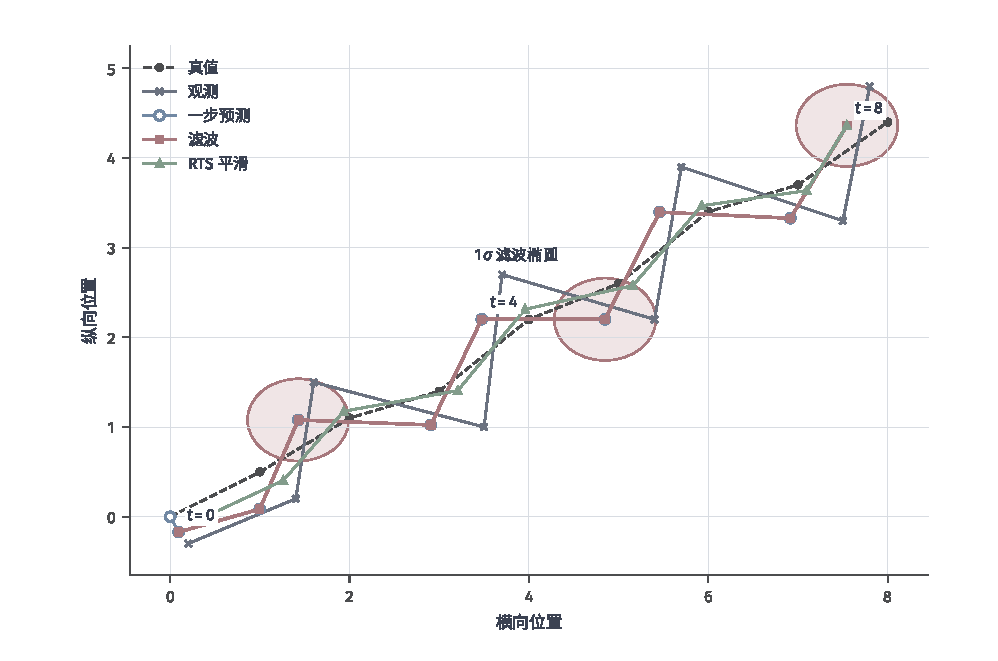
\includegraphics[width=159.059mm]{figures/06-probabilistic-graphical-models/04-models/matplotlib/pgm-dynamic-kalman-trajectory/figure.pdf}
  \caption{人工二维轨迹上的Kalman滤波与RTS平滑。黑色虚线为真值，灰叉为观测，蓝色空心点为观测前预测，红色方点为在线滤波均值，绿色三角为读取全部九次观测的平滑均值。红色半透明椭圆在$t=2,5,8$处显示滤波不确定性，其半轴为各坐标$1$倍标准差；末时刻两类均值重合。图源保存全部参数和坐标，结果对应这组固定的随机游走假设与观测。}
  \label{fig:pgm-dynamic-kalman-trajectory}
\end{figure*}

例~\ref{ex:pgm-dynamic-kalman}第二时刻的更新也可以直接看密度（图~\ref{fig:pgm-dynamic-gaussian}）。观测似然集中在$2$附近，预测密度集中在$0.5$附近，相乘并归一化后，后验均值位于$1.4$。测量与预测共同约束同一状态，使后验方差缩小。

\begin{figure}[htbp]
  \centering
  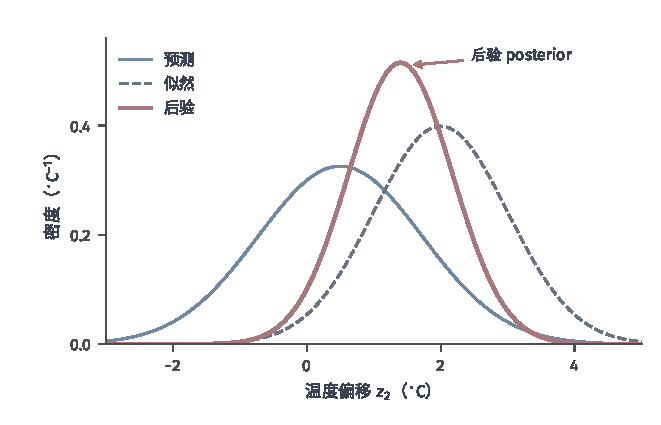
\includegraphics[width=105.412mm]{figures/06-probabilistic-graphical-models/04-models/matplotlib/pgm-dynamic-gaussian/figure.pdf}
  \caption{标量Kalman更新中的预测、似然与后验。蓝色实线表示预测$\mathcal{N}(0.5,1.5)$，灰色虚线表示对状态归一化的似然$\mathcal{N}(2,1)$，红色粗线表示后验$\mathcal{N}(1.4,0.6)$；引线对应各曲线。横轴为温度偏移，纵轴为密度。这里观测矩阵为$1$，观测似然对状态归一化后恰好形成图示高斯密度。}
  \label{fig:pgm-dynamic-gaussian}
\end{figure}

未知的线性映射和噪声协方差，可以用状态后验统计量来估计。线性高斯EM先计算完全数据对数似然需要的一阶、二阶矩，再拟合转移与观测分布。这与Baum--Welch按软计数学习的结构相同，区别在于连续状态用矩保存期望。当前参数下所需的统计量为
\begin{equation}
  \begin{aligned}
    \overline{\bm{z}}_t&=\bm{m}_{t\mid T},\\
    \bm{M}_t
      &:=\mathbb{E}[\bm{z}_t\bm{z}_t^\top\mid\bm{x}_{1:T}]
        =\bm{P}_{t\mid T}
          +\overline{\bm{z}}_t\overline{\bm{z}}_t^\top,\\
    \bm{M}_{t,t-1}
      &:=\mathbb{E}[\bm{z}_t\bm{z}_{t-1}^\top\mid\bm{x}_{1:T}]\\
      &=\bm{P}_{t,t-1\mid T}
          +\overline{\bm{z}}_t\overline{\bm{z}}_{t-1}^\top.
  \end{aligned}
  \label{eq:pgm-dynamic-em-moments}
\end{equation}
这些期望由同一组旧参数下的滤波和平滑结果给出，在整个M步中保持固定。Ghahramani和Hinton给出了线性系统EM的完全数据似然及相应充分统计量的推导\scite{pgm-dynamic-ghahramani1996}

M步怎样使用这些矩，可以从残差展开看出。记转移残差$\bm r_t(\bm A)=\bm z_t-\bm A\bm z_{t-1}$，其期望外积为
\begin{equation}
  \begin{aligned}
    \bm{E}_t(\bm{A})
      &:=\mathbb{E}\bigl[
        \bm r_t(\bm A)\bm r_t(\bm A)^\top
        \mid\bm{x}_{1:T}\bigr]\\
      &=\bm{M}_t-\bm{A}\bm{M}_{t,t-1}^{\top}
        -\bm{M}_{t,t-1}\bm{A}^{\top}\\
      &\quad{}+\bm{A}\bm{M}_{t-1}\bm{A}^{\top}.
  \end{aligned}
  \label{eq:pgm-dynamic-transition-residual}
\end{equation}
观测残差的期望外积$\bm{D}_t(\bm{C})$同样展开为
\[
  \begin{aligned}
    \bm{D}_t(\bm{C})
      &=\bm{x}_t\bm{x}_t^\top
        -\bm{C}\overline{\bm{z}}_t\bm{x}_t^\top
        -\bm{x}_t\overline{\bm{z}}_t^\top\bm{C}^\top\\
      &\quad{}+\bm{C}\bm{M}_t\bm{C}^\top.
  \end{aligned}
\]
转移与观测的高斯对数密度包含协方差行列式和加权残差二次型。将二次型写成迹、再取后验期望，EM辅助目标为
\begin{equation}
  \begin{aligned}
    \mathcal Q
      &=-\frac{T-1}{2}\log|\bm Q|
        -\frac12\sum_{t=2}^{T}
          \operatorname{tr}\{\bm Q^{-1}\bm E_t(\bm A)\}\\
      &\quad{}-\frac{T}{2}\log|\bm R|
        -\frac12\sum_{t=1}^{T}
          \operatorname{tr}\{\bm R^{-1}\bm D_t(\bm C)\}\\
      &\quad{}+\text{初始项}+\text{常数}.
  \end{aligned}
  \label{eq:pgm-dynamic-lgssm-q}
\end{equation}
辅助目标把M步分成线性回归和协方差估计。回归使用完整后验二阶矩，因此平滑均值之外的状态不确定性也进入残差与参数更新。

当$T\geq2$、观测完整且相关二阶矩和可逆时，对$\bm A$求导得到回归的正规方程
\[
  \bm A^{(k+1)}\sum_{t=2}^{T}\bm M_{t-1}
    =\sum_{t=2}^{T}\bm M_{t,t-1}.
\]
观测映射满足相同形式的回归方程。先更新两个映射，再用新映射计算期望残差，得到
\begin{equation}
  \begin{aligned}
    \bm A^{(k+1)}
      &=\left(\sum_{t=2}^{T}\bm M_{t,t-1}\right)
        \left(\sum_{t=2}^{T}\bm M_{t-1}\right)^{-1},\\
    \bm C^{(k+1)}
      &=\left(\sum_{t=1}^{T}
        \bm x_t\overline{\bm z}_t^\top\right)
        \left(\sum_{t=1}^{T}\bm M_t\right)^{-1},\\
    \bm Q^{(k+1)}
      &=\frac{1}{T-1}\sum_{t=2}^{T}
        \bm E_t(\bm A^{(k+1)}),\\
    \bm R^{(k+1)}
      &=\frac{1}{T}\sum_{t=1}^{T}
        \bm D_t(\bm C^{(k+1)}).
  \end{aligned}
  \label{eq:pgm-dynamic-lgssm-m-step}
\end{equation}
对$\bm Q^{-1}$或$\bm R^{-1}$求导即可得到协方差更新，例如转移项满足$(T-1)\bm Q=\sum_t\bm E_t$。单条序列的初始参数更新为$\bm m_0^{(k+1)}=\overline{\bm z}_1$、$\bm P_0^{(k+1)}=\bm P_{1\mid T}$。对$n$条独立序列，$\bm m_0^{(k+1)}$取初始平滑均值的平均，$\bm P_0^{(k+1)}$取各初始平滑协方差与初始均值相对总体均值外积之和的平均。转移残差按$\sum_{\ell=1}^{n}(T_\ell-1)$归一化，观测残差按$\sum_{\ell=1}^{n}T_\ell$归一化。初始协方差这样同时保存序列内部的不确定性和各序列起点之间的差异。

将例~\ref{ex:pgm-dynamic-kalman}的平滑结果代入，得到$M_1=0.4+0.8^2=1.04$、$M_2=0.6+1.4^2=2.56$及$M_{2,1}=0.2+1.4\times0.8=1.32$。旧参数$A=C=Q=R=1$下算出的这组矩，给出一次无约束M步：
\[
  \begin{aligned}
    A^{(k+1)}&=1.32/1.04=33/26,\\
    C^{(k+1)}&=(1\times0.8+2\times1.4)/(1.04+2.56)=1,\\
    Q^{(k+1)}&=2.56-1.32^2/1.04=23/26,\\
    R^{(k+1)}&=(1^2+2^2-3.6)/2=0.7.
  \end{aligned}
\]
初始均值与方差分别变为$0.8$和$0.4$。更新得到$A^{(k+1)}>1$，说明无约束极大化可以选择增长的动力学；只有两个观测时，全部系统参数的识别还缺少数据支持。若目标要求稳定动力学，可在$\bm A$的谱半径上施加约束，并求解对应M步。

每轮EM完成滤波、平滑和矩的累计，固定维度时成本随总序列长度线性增长。可以结合似然增量与迭代上限停止，并比较多组初值的观测预测。二阶矩和奇异时，回归可能有多个解；协方差落到退化边界时，需要处理低维支撑。协方差下界、先验、已知噪声结构或固定参数可以约束这些问题，对应目标和更新也随之改变。

连续状态的坐标也有等价表示。对任意可逆矩阵$\bm H$，改用$\widetilde{\bm z}_t=\bm H\bm z_t$，并同时变换$\widetilde{\bm A}=\bm H\bm A\bm H^{-1}$、$\widetilde{\bm C}=\bm C\bm H^{-1}$、$\widetilde{\bm Q}=\bm H\bm Q\bm H^\top$和初始分布，观测分布保持不变。把某个坐标解释成温度或磨损程度，需要测量关系等额外约束。若一个非零方向始终不被$\bm C,\bm C\bm A,\ldots$观测到，数据对该方向的约束还可能不足。因此，后验计算、状态识别和长期误差控制分别依赖相应的模型条件。

升温、恒温和冷却可能各自近似线性，却使用不同的转移参数。\term{切换线性动态系统}（switching linear dynamical system, SLDS）引入离散模式$S_t\in\{1,\ldots,L\}$，按模式选择连续转移与观测机制。这里$S_t$表示运行模式，与四节点例中传感器失灵变量$S$分别定义。一个常见形式为
\begin{equation}
  \begin{aligned}
    p(s_t\mid s_{t-1})&=\omega_{s_{t-1},s_t},\\
    \bm z_t\mid\bm z_{t-1},s_t
      &\sim\mathcal N(\bm A_{s_t}\bm z_{t-1},\bm Q_{s_t}),\\
    \bm x_t\mid\bm z_t,s_t
      &\sim\mathcal N(\bm C_{s_t}\bm z_t,\bm R_{s_t}),
  \end{aligned}
  \label{eq:pgm-dynamic-switching}
\end{equation}
指定$p(s_1)$与条件高斯初始分布$p(\bm z_1\mid s_1)=\mathcal N(\bm z_1;\bm m_{0,s_1},\bm P_{0,s_1})$后，就能按这些局部机制生成完整序列。图~\ref{fig:pgm-dynamic-switching}显示模式对连续状态与观测的影响。推断时模式也未知，需同时保留可能模式与各模式下的状态不确定性。

\begin{figure}[htbp]
  \centering
  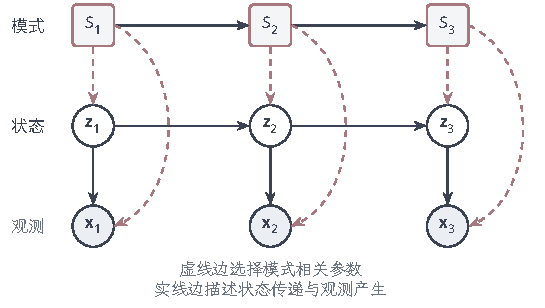
\includegraphics[width=92.276mm]{figures/06-probabilistic-graphical-models/04-models/tikz/pgm-dynamic-switching/figure.pdf}
  \caption{切换系统的三层依赖。方形节点表示离散模式，空心圆表示连续状态，填色圆表示观测。每条完整模式路径对应一组线性高斯递推；到达相同当前模式的不同历史仍可产生不同高斯后验。}
  \label{fig:pgm-dynamic-switching}
\end{figure}

固定模式历史$s_{1:t}$时，连续状态后验为高斯；换一条历史，均值和协方差一般随之改变。精确滤波把这些历史加在一起，最多形成$L^t$个高斯分量。合并、剪枝或限制每种当前模式的分量数，以近似换取可控成本。EM同时需要模式转移期望计数与各模式的连续二阶矩，E步的混合推断质量因而直接影响学习。

非线性动力学以及偏斜、离群点或离散跳变等噪声特征，可以用更一般的状态空间模型表示。具有加性噪声结构时，写为
\begin{equation}
  \bm z_t=f_t(\bm z_{t-1})+\bm\varepsilon_t,\qquad
  \bm x_t=h_t(\bm z_t)+\bm\eta_t.
  \label{eq:pgm-dynamic-nonlinear}
\end{equation}
直接指定转移和观测分布，还可以表示非加性、非高斯机制。Bayes递推式~\eqref{eq:pgm-dynamic-bayes-filter}依然适用，但单个高斯通常无法精确保存更新后的后验。下列方法分别在局部函数、积分矩或路径后验上近似，由此保留不同的信息。

在当前估计附近用一阶线性函数近似动力学和观测函数，就可以继续传播高斯均值与协方差。这形成\term{扩展Kalman滤波}（extended Kalman filter, EKF）。对加性高斯噪声，记$\bm F_t$为$f_t$在$\bm m_{t-1\mid t-1}$处的Jacobian，$\bm H_t$为$h_t$在预测均值处的Jacobian，预测计算为
\[
  \begin{aligned}
    \bm m_{t\mid t-1}&\approx f_t(\bm m_{t-1\mid t-1}),\\
    \bm P_{t\mid t-1}
      &\approx\bm F_t\bm P_{t-1\mid t-1}\bm F_t^\top+\bm Q_t,\\
    \bm S_t&\approx\bm H_t\bm P_{t\mid t-1}\bm H_t^\top+\bm R_t.
  \end{aligned}
\]
观测更新以$h_t(\bm m_{t\mid t-1})$为预测读数，以$\bm P_{t\mid t-1}\bm H_t^\top\bm S_t^{-1}$为增益。函数可微、后验集中在线性化有效区域时，局部函数及其矩的近似较为适用。初值偏离、强曲率或分离的后验峰会削弱这种局部表示。

也可以让少量代表点直接经过非线性函数，用输出点估计变换后的矩。\term{无迹变换}（unscented transform, UT）选择确定性点来匹配输入均值与协方差，因而省去Jacobian计算。给定$q$维高斯近似$\mathcal N(\bm m,\bm P)$，取$\bm L\bm L^\top=\bm P$、$\kappa>0$，一种$2q+1$点规则为
\[
  \begin{aligned}
    \bm\chi_0&=\bm m,&w_0&=\frac{\kappa}{q+\kappa},\\
    \bm\chi_i&=\bm m+\sqrt{q+\kappa}\bm L_{:,i},
      &w_i&=\frac{1}{2(q+\kappa)},\\
    \bm\chi_{q+i}&=\bm m-\sqrt{q+\kappa}\bm L_{:,i},
      &w_{q+i}&=\frac{1}{2(q+\kappa)},
  \end{aligned}
\]
这里$i=1,\ldots,q$。对称点及其权重恰好恢复输入的$\bm m,\bm P$。经过$f$后，加权均值$\widehat{\bm\mu}=\sum_iw_i f(\bm\chi_i)$和协方差$\sum_iw_i(f(\bm\chi_i)-\widehat{\bm\mu})(f(\bm\chi_i)-\widehat{\bm\mu})^\top$近似输出矩。将这一规则用于预测状态、预测观测和两者的交叉协方差，再按高斯分布条件化，得到\term{无迹Kalman滤波}（unscented Kalman filter, UKF）。

例如$Z\sim\mathcal N(0,1)$经过$f(Z)=Z^2$。在$0$处，函数值和导数均为$0$，EKF给出的均值、方差都是$0$，精确结果则为$1$和$2$。取$q=1,\kappa=2$，代表点$0,\sqrt3,-\sqrt3$对应权重$2/3,1/6,1/6$，输出为$0,3,3$，加权后恰好恢复均值$1$、方差$2$。这个例子展示了代表点怎样捕捉均值附近的曲率。对其他函数，积分矩仍有近似误差；UKF还将条件后验压缩成一个高斯，分离的多个峰因此会丢失。Särkkä和Svensson讨论了EKF、UT及平滑扩展的条件与算法\scite{pgm-dynamic-sarkka2023}

整段状态重建或参数学习还可以直接近似路径后验。\term{变分状态估计}（variational state estimation）选择可计算的路径分布$q_{\bm\phi}(\bm z_{1:T})$，通过最大化证据下界拟合它（第~\ref{chap:pgm-variational}章）。在线性或局部二次近似下，结构化高斯族可保留相邻时刻的相关性；切换系统也可用离散模式链和连续状态链联合表示。近似族确定了哪些依赖和后验形状能够保存。联合学习时，下界由观测对数似然和近似后验误差共同决定，优化过程中两者都可能变化；模型的预测表现仍需单独评价。

分离的后验峰对应不同状态解释，可以用一组样本同时保留。\term{粒子滤波}（particle filtering）以带权状态样本近似滤波分布。设粒子数$n$，第$i$个粒子为$\bm z_{t,i}$，按$q_t(\bm z_t\mid\bm z_{t-1,i},\bm x_t)$提议。在尚未重采样的一步，权重更新为
\[
  w_{t,i}\propto w_{t-1,i}
    \frac{p(\bm x_t\mid\bm z_{t,i})
      p(\bm z_{t,i}\mid\bm z_{t-1,i})}
      {q_t(\bm z_{t,i}\mid\bm z_{t-1,i},\bm x_t)}.
\]
若先按旧权重重采样祖先，祖先选择已计入旧权重，新权重只需当前的重要性比率。序贯重要性更新及带重采样的自举滤波见式~\eqref{eq:pgm-sampling-sis-weight}与算法~\ref{alg:pgm-sampling-bootstrap}。它们用样本和加权和代替难以解析的积分。转移先验提议可约去权重中的转移项；观测集中时，却可能让大量粒子落在低似然区域。每步需要约$n$次转移、似然求值以及重采样，维度与时间跨度影响所需粒子数。固定$n$时，应检查权重集中和样本覆盖。

在式~\eqref{eq:pgm-dynamic-switching}中，可以只抽样离散模式路径，每个粒子内部按给定模式历史运行精确Kalman递推。这种Rao--Blackwell化利用条件线性高斯结构来减少采样对象（第~\ref{chap:pgm-sampling}章）。长期重采样可能使许多粒子共享早期祖先，降低过去路径的多样性。因此，离线平滑和EM还需粒子平滑或其他路径后验方法，计算选择取决于任务需要保留的状态或路径不确定性。

\section{模型比较}
\label{sec:pgm-dynamic-comparison}

比较动态模型时，先固定要描述的状态与要回答的查询：状态是否可见、取离散值还是连续值，转移保留多长历史，推断可读取哪些时刻的证据。表~\ref{tab:pgm-dynamic-models}据此并列各类模型的条件和计算。DBN作为共同表示框架适用于各行，具体差别来自状态空间、局部分布和依赖假设。

\begin{table*}[htbp]
  \centering
  \small
  \begin{tabularx}{\linewidth}{@{}p{25mm}p{23mm}p{29mm}p{27mm}X@{}}
    \toprule
    模型 & 状态可见性与空间 & 转移假设 & 常见查询 & 推断与学习 \\
    \midrule
    有限Markov链 & 可见、离散 & 按当前状态给出下一状态分布 & 多步预测、长期分布 & 矩阵递推；可见转移计数 \\
    HMM & 隐藏、离散 & 一阶链，几何停留时间 & 滤波、平滑、整条路径 & 前向--后向、Viterbi；Baum--Welch \\
    高阶HMM与HSMM & 隐藏、离散或分段状态 & 更长历史或显式持续时间 & 路径与片段边界 & 扩充状态或片段动态规划；期望计数 \\
    因子HMM & 多条隐藏离散链 & 先验转移分开，观测耦合 & 联合滤波与平滑 & 联合表可精确但指数增长；变分或采样 \\
    线性高斯模型 & 隐藏、连续 & 线性转移与独立高斯噪声 & 状态分布、预测密度 & Kalman滤波、RTS平滑；二阶矩EM \\
    切换线性系统 & 隐藏、离散与连续混合 & 模式选择线性动态 & 模式与连续状态联合查询 & 高斯混合枚举一般指数增长；混合约简或条件粒子方法 \\
    一般状态空间模型 & 隐藏、连续或混合 & 非线性、非高斯等 & 滤波、平滑及预测风险 & 局部线性化、矩近似、变分或粒子方法 \\
    \bottomrule
  \end{tabularx}
  \caption{动态有向模型的状态、转移与计算。各类模型均需指定初始分布，线性高斯精确递推还需高斯初态。近似方法可按后验形状和查询要求组合选择。}
  \label{tab:pgm-dynamic-models}
\end{table*}

有限状态动态规划和Kalman递推每次都将过去压缩成固定大小的精确消息。前者保存$K$个状态概率，后者保存均值向量和协方差矩阵，因而维度固定时，总成本随时间长度线性增长。接口固定仍可能带来昂贵消息：因子HMM需记录$K^M$种联合配置，切换系统的高斯分量又随模式历史增多。评价成本时，应同时给出序列长度、接口维度和消息表示。

证据可用的时刻决定查询算法。在线控制按当前和过去读数滤波，事后检修则可借助未来证据平滑，两者应分别评价。若损失按逐时刻误判数累计，平滑边缘给出相应最优决策；要求完整路径满足转移限制时，则优化联合解释。连续联合高斯后验的均值也是联合密度众数，混合后验中这两个对象却可能分离，平均值甚至位于分量之间的低密度区域。

误差诊断需要同时检查模型和计算。HMM即使精确推断，也可能因状态过少或持续时间假设偏差而预测失配；EKF还增加了局部线性化误差。比较方法时，固定训练与测试的时间边界，以及一步或多步预测目标，再报告预测对数密度与计算成本；有状态参考值时，可同时评价状态误差和后验不确定性覆盖。按时间保持数据边界，才能评价面向未来的预测；打乱时间点或提前读取未来观测会改变这个任务。

共享参数把多个时刻的数据用于估计同一局部机制，在共享假设适用时减少了待估自由度。运行环境变化后，旧的齐次机制可能失配；已知输入、时变参数或模式切换可表示这种变化，新增机制也需要相应数据来识别。选择模型时，先确定任务所需依赖，再检查状态后验的表示与计算成本，使表达范围、可估计性和推断方法相互匹配。

\section{本章小结}
\label{sec:pgm-dynamic-summary}

动态有向分解把过去对未来的影响集中到时间接口上，使新观测能够逐步并入当前判断。DBN规定依赖模板，Markov性规定给定状态后哪些历史可被压缩，时间齐次与参数共享规定机制的复用方式，平稳性规定过程分布在时间平移下的变化。明确各项条件，才能知道递推中保存的消息代表什么。

有限隐藏状态用前向--后向消息累加路径概率，用Viterbi前驱表恢复最优路径，再由Baum--Welch按后验期望计数学习。线性高斯系统用均值和协方差精确保存状态分布，经Kalman滤波与RTS平滑取得一阶、二阶矩，再拟合局部映射与噪声。这两条路线都先以局部消息完成全局推断，再把后验统计量交给参数学习。

设备的当前报警判断、故障追溯和整段工况解释分别对应滤波、平滑和路径查询。状态增多、持续时间复杂或模式与连续动态混合时，精确消息成本上升，局部高斯、变分和粒子方法在不同位置近似。模型的表达假设决定可描述的演化规律，推断与学习决定怎样从观测取得判断，时间隔离的预测评价则检验它在新数据上的适用性。

\paragraph{扩展阅读}
Bishop的PRML第13章从顺序数据展开HMM与线性动态系统，Murphy的教材进一步讨论滤波、平滑和状态估计。阅读时可沿同一观测序列比较各查询的证据范围，并追踪后验消息怎样变成参数学习所需的统计量\scite{bishop2006,pgm-murphy2012}
